% 
% Information Retrieval
% -------------------------------
% University of California Irvine
% 
% Author:
% - María Carrasco Rodríguez
% - Fabs Lindenberg
% - Lea Voget

\documentclass[a4paper,11pt,oneside]{book}
\usepackage{wrapfig} 
\usepackage{helvet}
\usepackage{phdthesis}
\usepackage{kostspielig}
\usepackage{amsmath}
\usepackage{multirow}
\usepackage{colortbl}
\usepackage{appendix}
\usepackage{pifont}
\usepackage{color}
\usepackage{amsmath}
\usepackage{epsfig}


%\pagestyle{fancy}
%\fancyhead{}
%\fancyhead[L]{\textsf{\textbf{CS 221 Information Retrieval}\\ Assignment 2}}
%\fancyhead[R]{\textsf{Maria Carrasco (16874129)\\ Fabian Lindenberg (74076658)}}
%\fancyfoot[R]{\textsf{\thepage}}
%\renewcommand{\footrulewidth}{0.4pt}
%\cfoot[]{}


\newcommand{\todo}[1]{\textcolor{red}{\textbf{TODO: #1}}}

\hypersetup{colorlinks, 
           linkbordercolor= 1 0.8 0.8,
           citecolor=black,
           filecolor=black,
           linkcolor=black,
           urlcolor=black,
           bookmarksopen=true,
           pdftex}
\title{Information Retrieval }
\subtitle{Assignment 5}
\location{University of California Irvine}
\author{ María Carrasco Rodríguez (16874129) \\
		Fabian Lindenberg (74076658)\\
		Lea Voget (45869178)}



\begin{document}

\kostspieligmaketitle

%\tableofcontents
%\pagebreak
% \startapendix

\setcounter{chapter}{1}
\chapter{Quantification of the Dataset}

\begin{enumerate}
	\item \begin{enumerate}
					\item The total of all unfiltered and unprocessed words in the document was 1456106.
					\item Each book had the following number of words. \emph{Emma}: 165075, \emph{Anna Karenina}: 361786, \emph{Jane Eyre}: 192539, \emph{Moby Dick}: 221810,  \emph{Portrait of a Lady}: 246057, \emph{Pride and Prejudice}: 125969 % TODO: two volumes of portrait of a lady?
					\item The word ``love'' appeared 983 times in the whole corpus and ``adventure'' occurred 19 times. 
								
								The number of occurences of these words per book are:
								\begin{itemize}
									\item Anna Karenina:
												\begin{itemize}
													\item{love:	433}
													\item{adventure:	0}
												\end{itemize}
									\item Emma:
												\begin{itemize}
													\item{love:	117}
													\item{adventure:	2}
												\end{itemize}
									\item Jane Eyre:
												\begin{itemize}
													\item{love:	151}
													\item{adventure:	3}
												\end{itemize}
									\item Moby Dick:
												\begin{itemize}
													\item{love:	24}
													\item{adventure:	5}
												\end{itemize}
									\item Portrait of a Lady:
												\begin{itemize}
													\item{love:	146}
													\item{adventure:	7}
												\end{itemize}
									\item Pride and Prejudice:
												\begin{itemize}
													\item{love:	92}
													\item{adventure:	2}
												\end{itemize}
									\item Three Men in a Boat:
												\begin{itemize}
													\item{love:	10}
													\item{adventure:	0}
												\end{itemize}
								\end{itemize}
					\item The books \emph{Anna Karenina} and \emph{Three men in a boat} did not contain the word ``adventure''
					\item The top 5 (stemmed) words in each book were:
								\begin{itemize}
									\item Anna Karenina:
												\begin{itemize}
													\item{levin:		1629}
													\item{vronski:	865}
													\item{anna:	825}
													\item{well:		675}
													\item{kitti:		672}
												\end{itemize}
									\item Emma:
												\begin{itemize}
													\item{emma:	867}
													\item{harriet:	506}
													\item{thing:	462}
													\item{weston:	448}
													\item{elton:	408}
												\end{itemize}
									\item Jane Eyre:
												\begin{itemize}
													\item{rochest:	371}
													\item{jane:		348}
													\item{well:		348}
													\item{sir:	315}
													\item{dai:	308}
												\end{itemize}
									\item Moby Dick:
												\begin{itemize}
													\item{whale:	1629}
													\item{ship:		623}
													\item{sea:		542}
													\item{man:		540}
													\item{ahab:	512}
												\end{itemize}
									\item Portrait of a Lady:
												\begin{itemize}
													\item{isabel:	1490}
													\item{don:		833}
													\item{ve:		683}
													\item{osmond:	588}
													\item{ralph:	578}
												\end{itemize}
									\item Pride and Prejudice:
												\begin{itemize}
													\item{elizabeth:	635}
													\item{darci:	417}
													\item{bennet:	333}
													\item{binglei:	311}
													\item{sister:	294}
												\end{itemize}
									\item Three Men in a Boat:
												\begin{itemize}
													\item{harri:		275}
													\item{georg:	263}
													\item{boat:		231}
													\item{work:	164}
													\item{river:	162}
												\end{itemize}
								\end{itemize}
					\end{enumerate}
						

%Total words of emma.txt is 
%The word love occured 117 times.
%The word adventure occured 2 times.
%the top 5 words are: 
%
%
%Total words of annaKarenina.txt is 
%The word love occured 433 times.
%The word adventure occured 0 times.
%the top 5 words are: 
%
%
%Total words of janeEyre.txt is 
%The word love occured 151 times.
%The word adventure occured 3 times.
%the top 5 words are: 
%
%
%Total words of mobyDick.txt is 0
%The word love occured 24 times.
%The word adventure occured 5 times.
%the top 5 words are: 
%
%
%Total words of portraitOfALady.txt is  
%The word love occured 146 times.
%The word adventure occured 7 times.
%the top 5 words are: 
%
%
%Total words of prideAndprejudice.txt is 
%The word love occured 92 times.
%The word adventure occured 2 times.
%the top 5 words are: 
%
%
%Total words of threeMenInABoat.txt is 71435
%The word love occured 10 times.
%The word adventure occured 0 times.
%the top 5 words are: 
%
%
%The word love occured 
%the top 5 words are: 
%time	2621
%thought	2166
%good	2283
%well	2423
%man	2280


	\item In order to quantify the books, we wrote a quantifier. The quantifier removes the header in front of each book and then tokenizes the content of the book. Counting the number of tokens, the total number of unprocessed words is calculated.
The quantifier has a hashmap that maps all words to their number of occurences
Then all tokens are stemmed and it is checked if they are stop words or not. If they are not stop words, they are either added to the \texttt{HashMap} or, if already present, their respective value is increased by one.
Finally, the quantifier searches for the five highest values and emits the five appropriate key-value pairs.

In order to find the number of occurences of ``love'' and ``adventure'', we did not use the stemmed version. Each token was checked if it was ``love'' or ``adventure'' just before stemming it.

The total number of words and of occurences of ``love'' and ``adventure'' in all books was found through giving the quantifier all book files at the same time.

We found out that some books did not contain ``love'' or ``adventure'', when the quantifier emitted that one of the words was found 0 times.
	\item We used the online tool \emph{Wordle} (\url{www.wordle.net}) to generate the word clouds of each book. We chose the following settings:
				\begin{itemize}
					\item case insensitivity (i.e. all words were transformed to their lowercase representation)
					\item remove common English words (according to a stop word list built into the tool)
					\item align the words mostly horizontally (for higher readability)
					\item black font color only (instead of using multiple different colors without meaning)
				\end{itemize} 
				The following figures show the resulting word clouds.
				\begin{figure}[htb]
					\begin{center}
					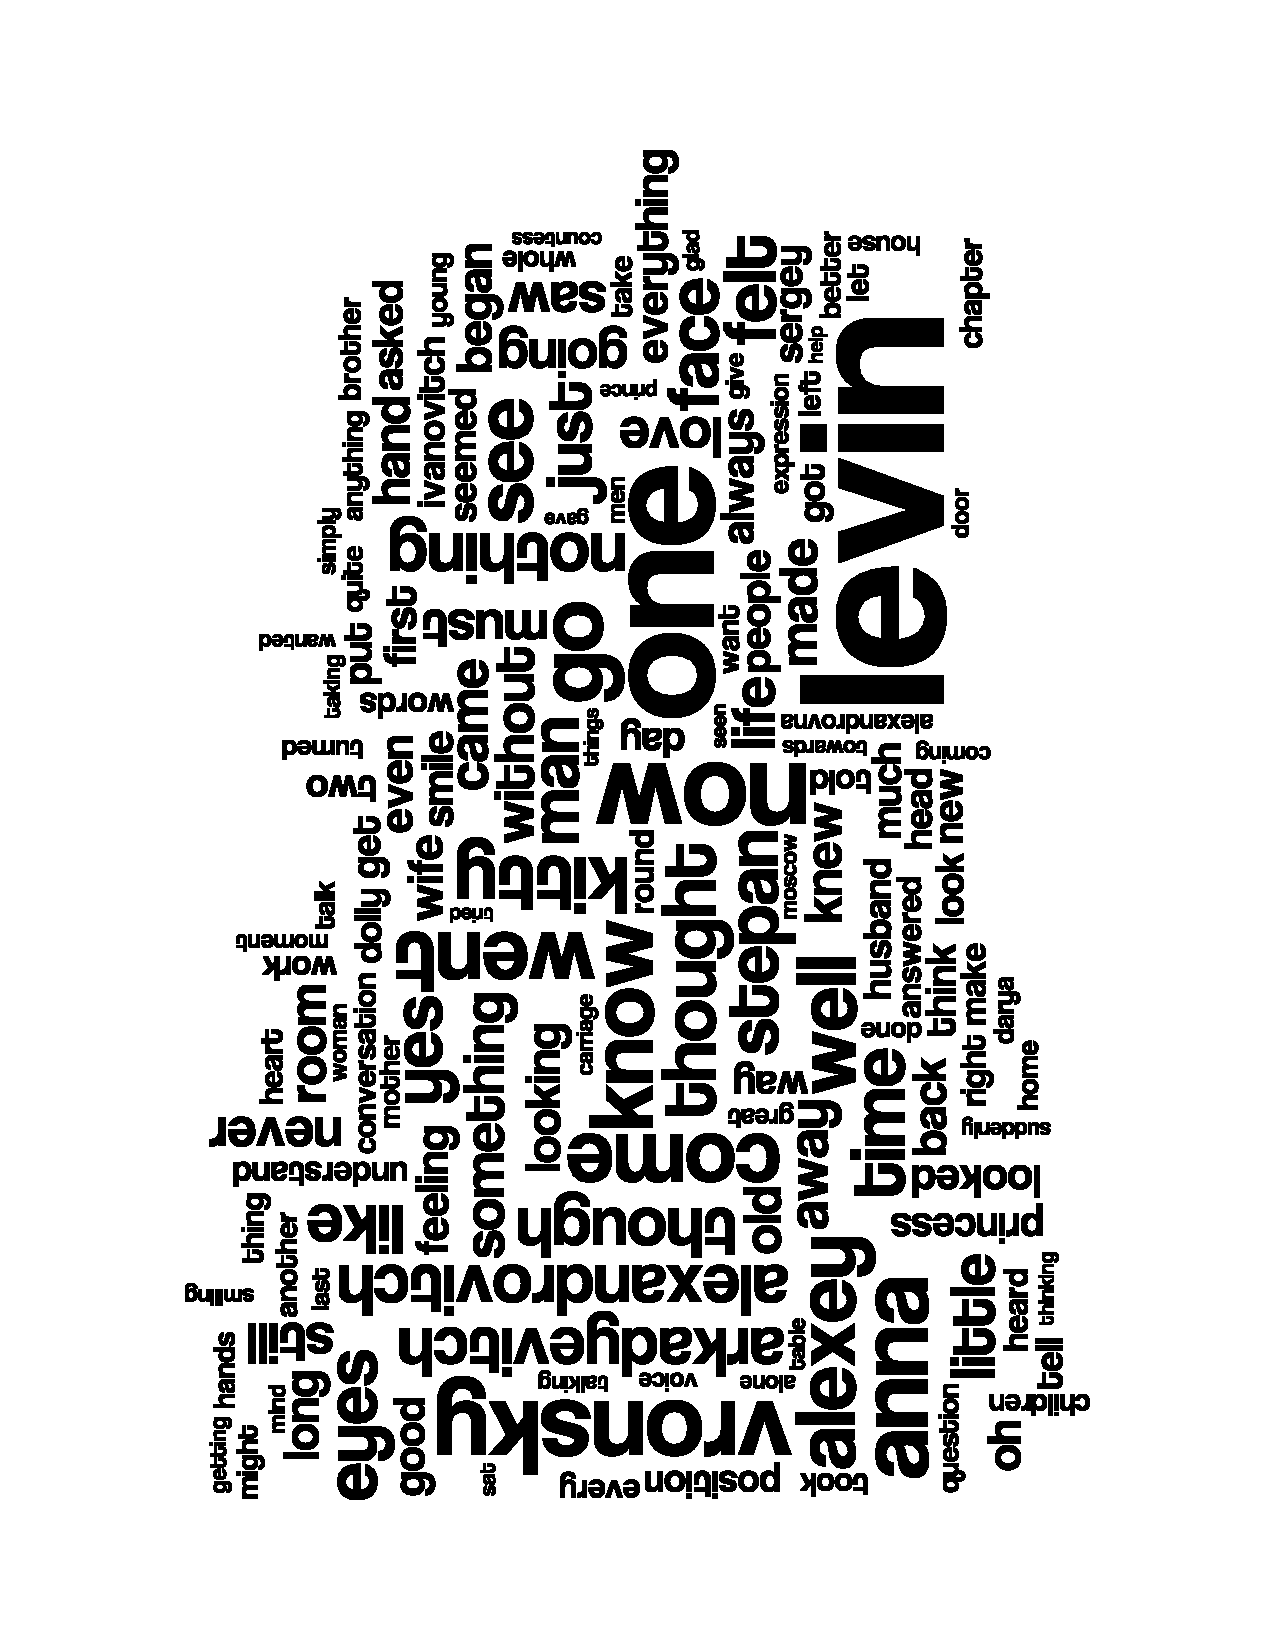
\includegraphics[angle=270,width=0.8\columnwidth]{resources/wordclouds/AnnaKarenina_WordCloud.pdf}%
					\end{center}
					\caption{Word cloud for \emph{Anna Karenina}}%
					\label{wcAnna}%
				\end{figure}
				\begin{figure}[htb]
					\begin{center}
					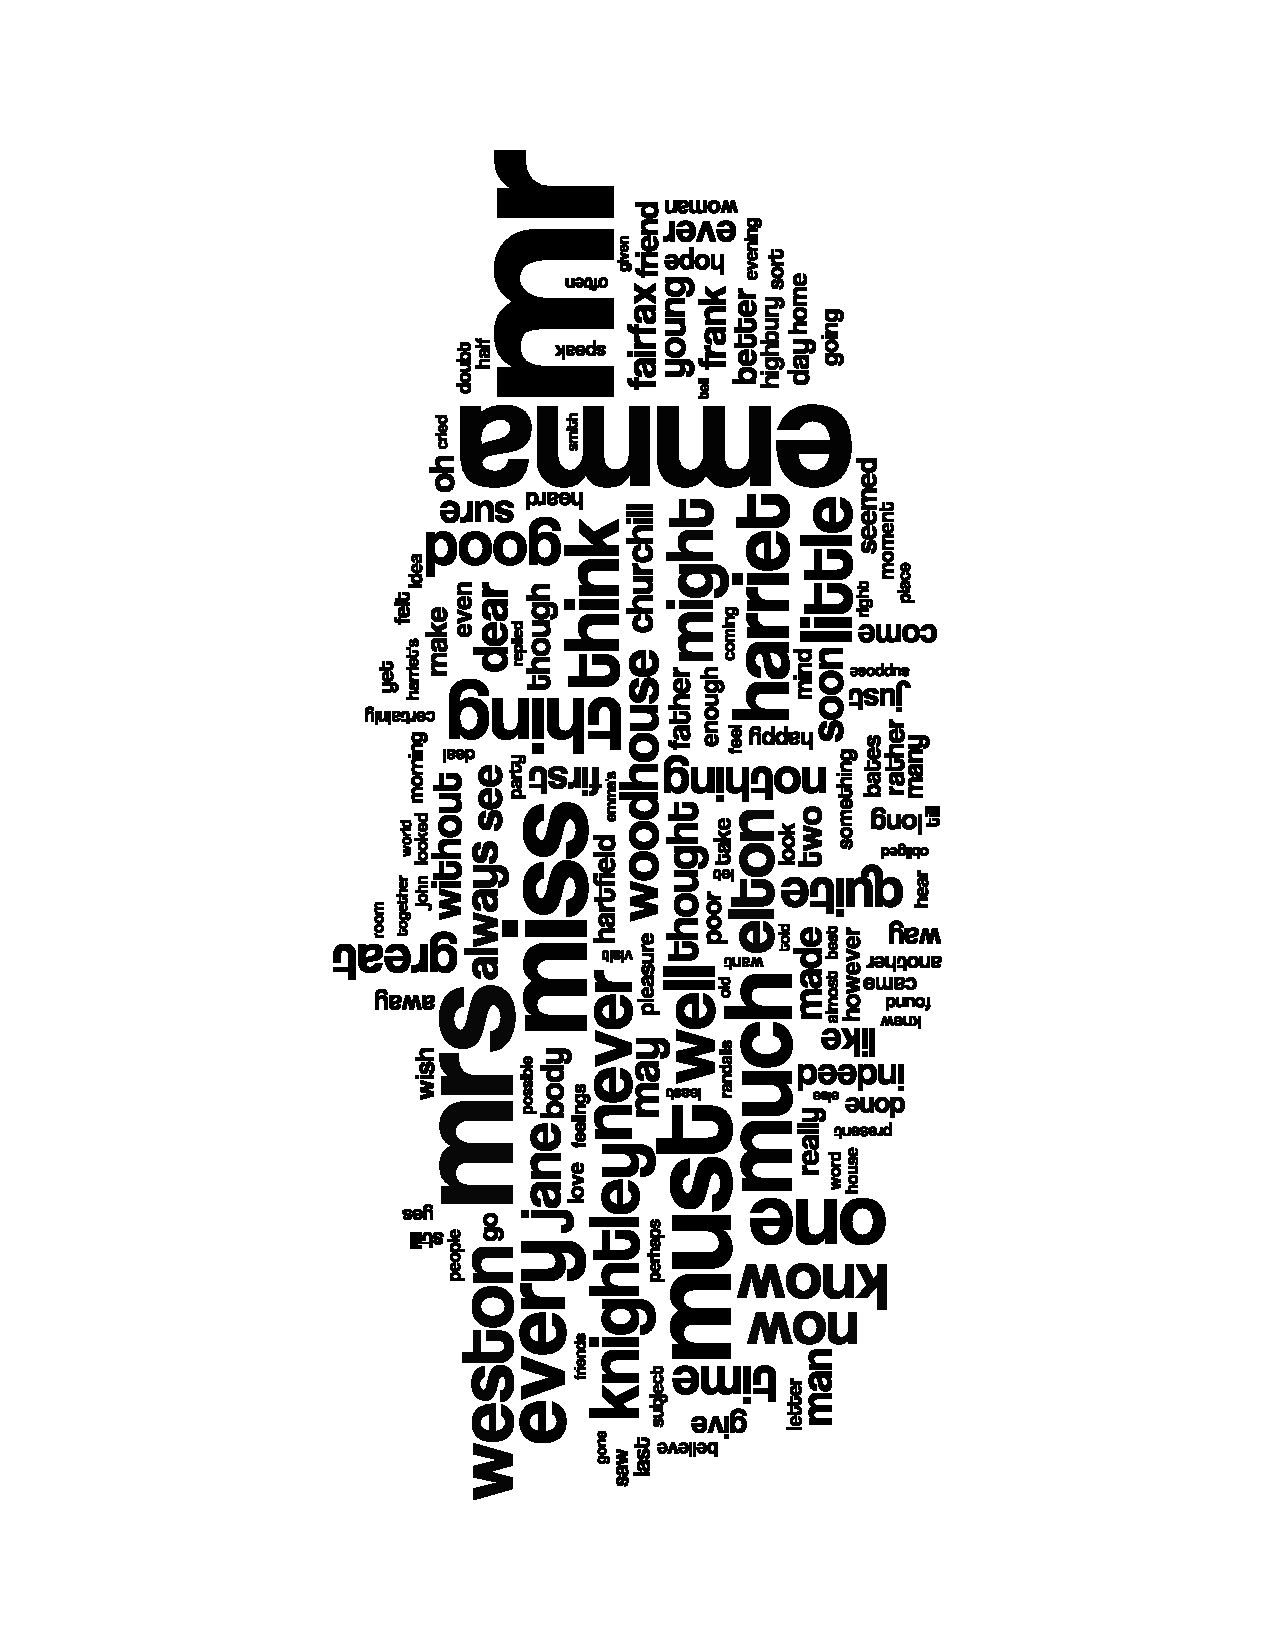
\includegraphics[angle=270,width=0.8\columnwidth]{resources/wordclouds/Emma_WordCloud.pdf}%
					\end{center}
					\caption{Word cloud for \emph{Emma}}%
					\label{wcEmma}%
				\end{figure}
				\begin{figure}[htb] 
					\begin{center}
					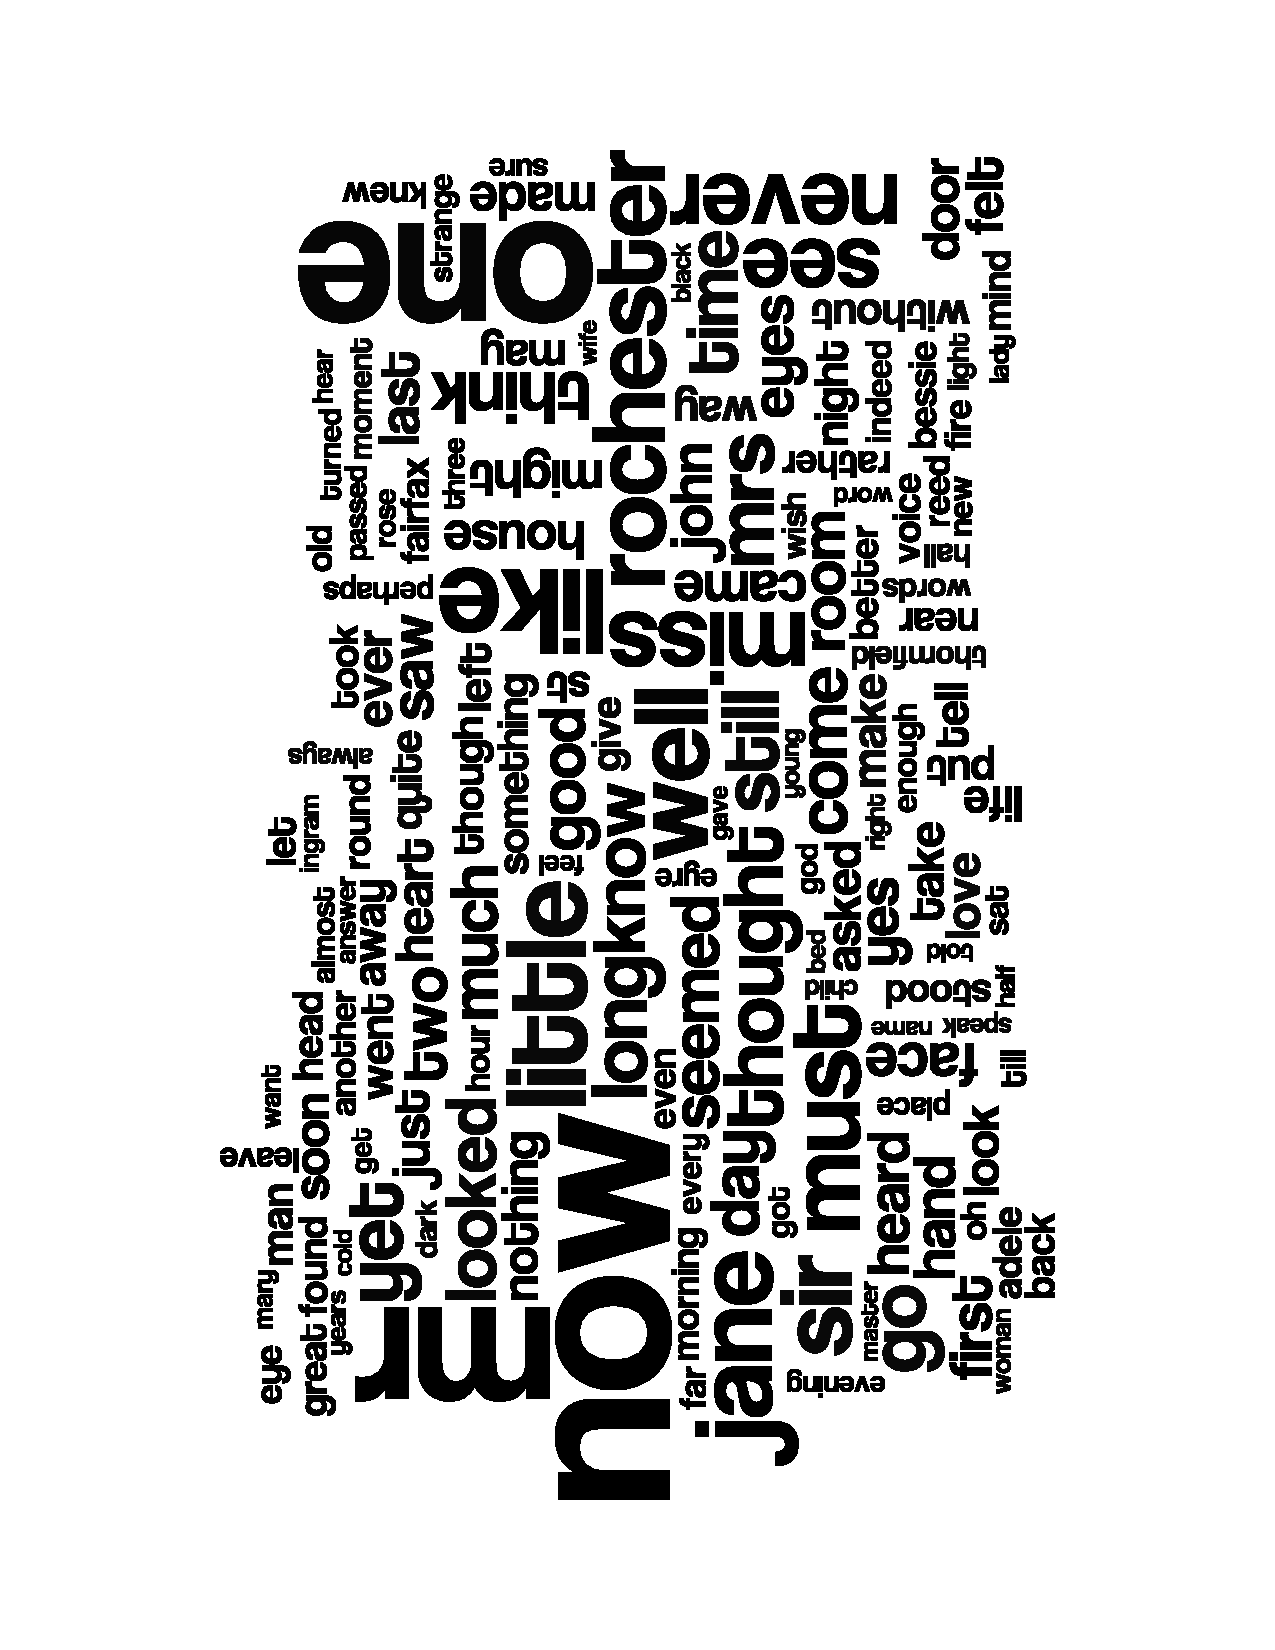
\includegraphics[angle=270,width=0.8\columnwidth]{resources/wordclouds/JaneEyre_WordCloud.pdf}%
					\end{center}
					\caption{Word cloud for \emph{Jane Eyre}}%
					\label{wcJane}%
				\end{figure}
				\begin{figure}[htb] 
					\begin{center}
					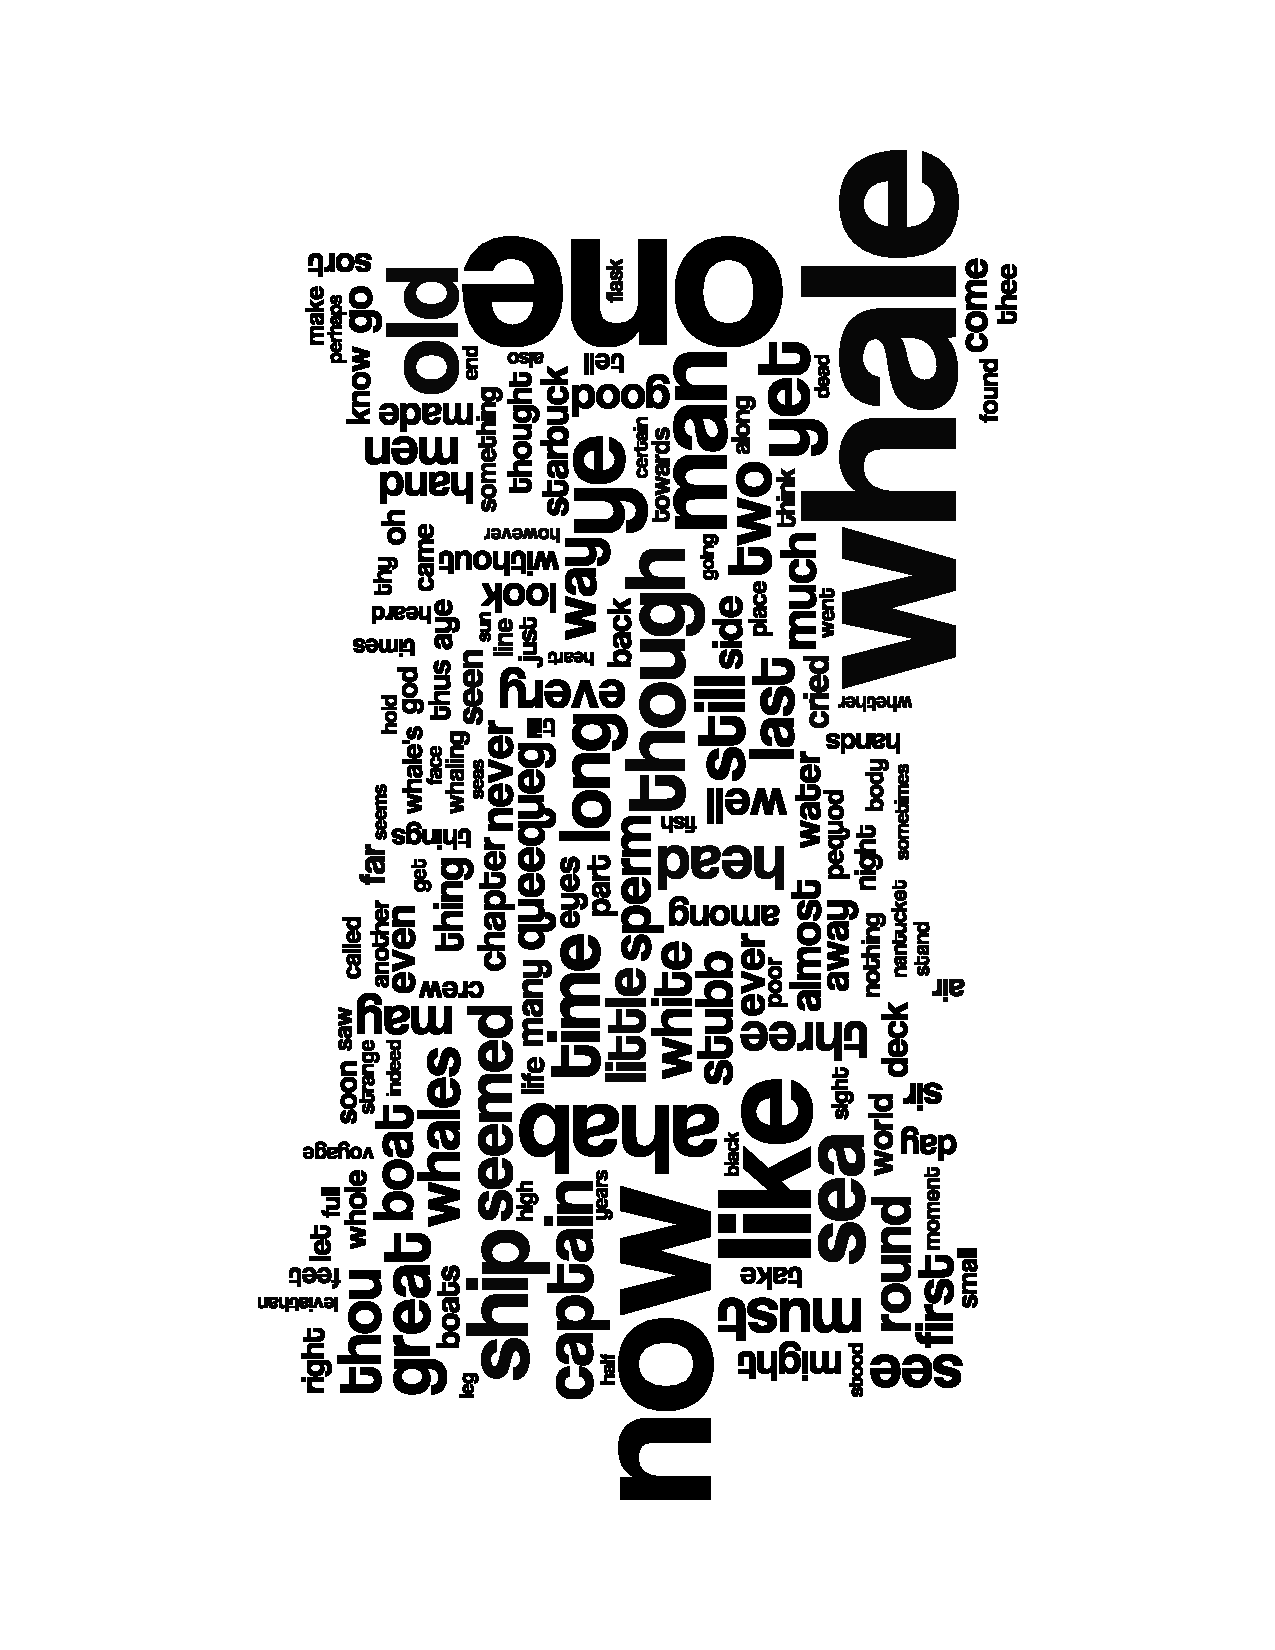
\includegraphics[angle=270,width=0.8\columnwidth]{resources/wordclouds/MobyDick_WordCloud.pdf}%
					\end{center}
					\caption{Word cloud for \emph{Moby Dick}}%
					\label{wcMoby}%
				\end{figure}
				\begin{figure}[htb] 
					\begin{center}
					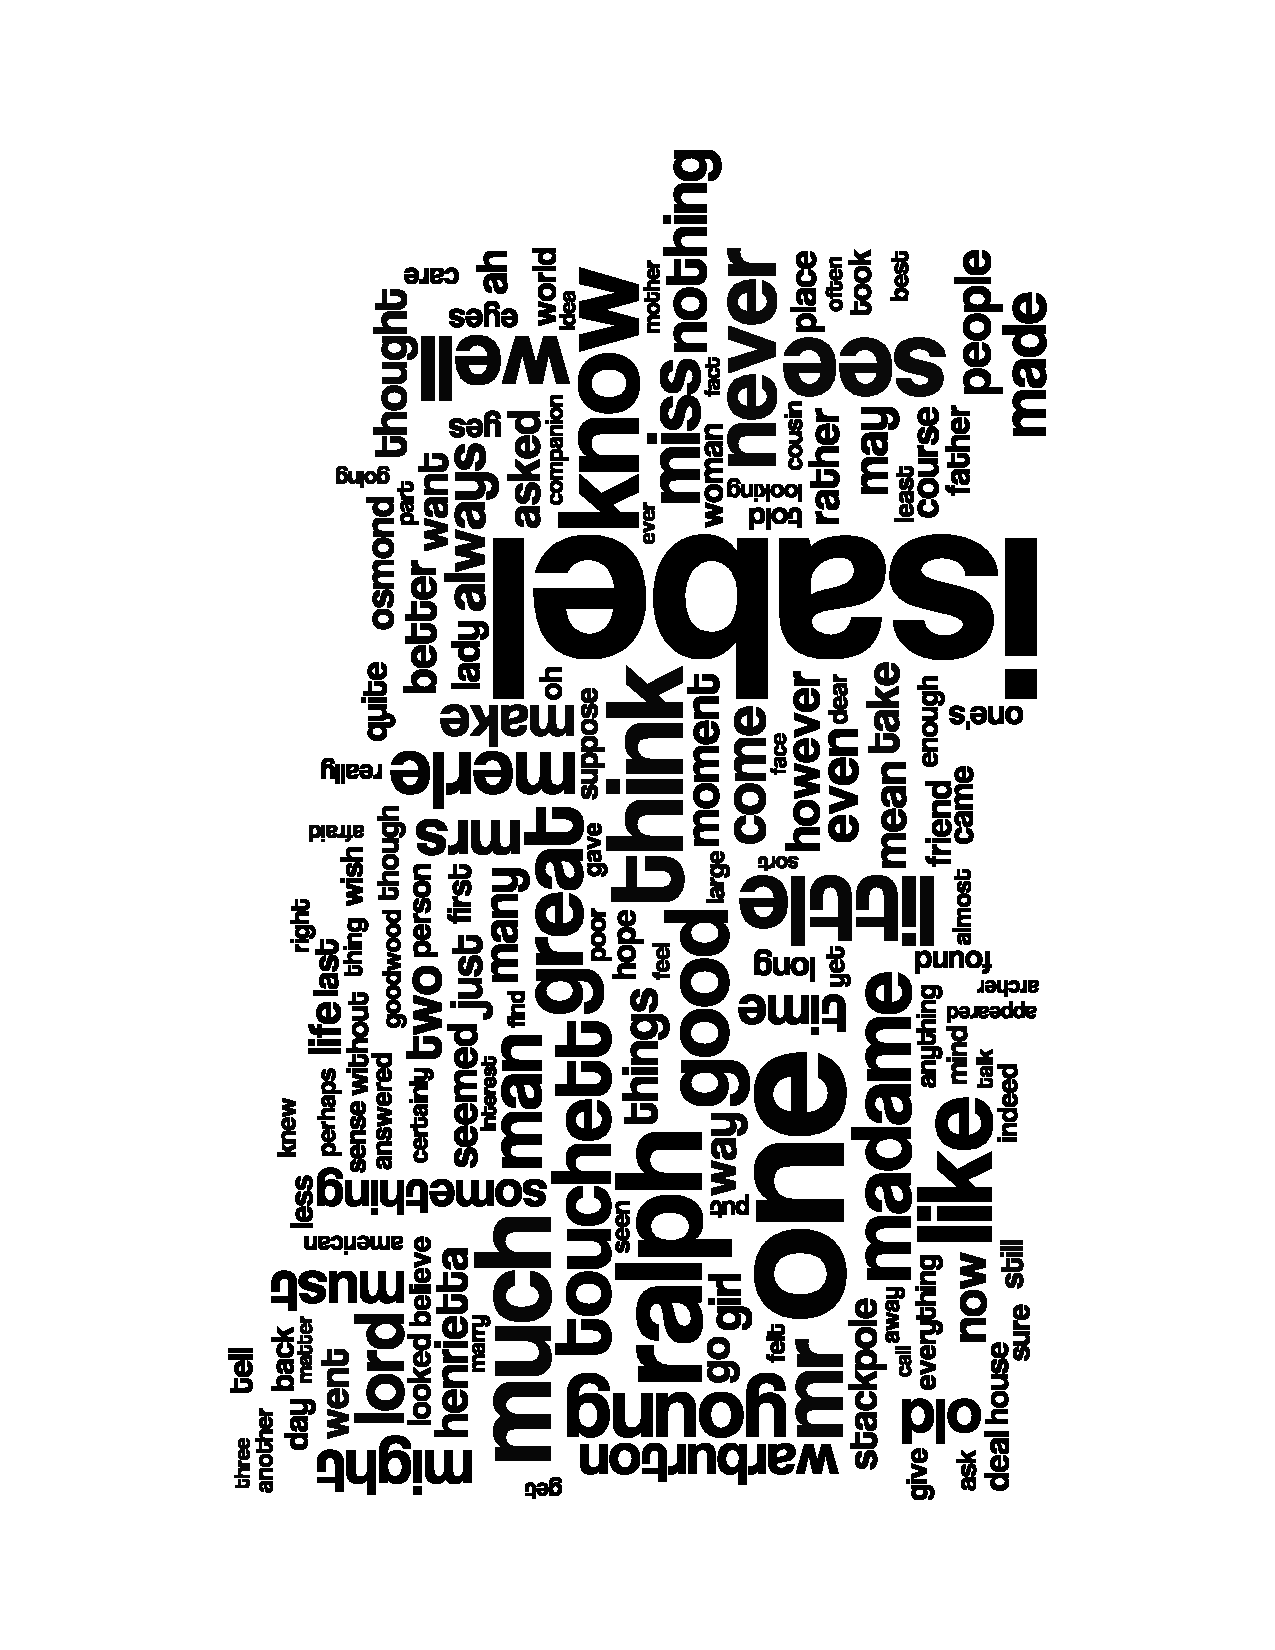
\includegraphics[angle=270,width=0.8\columnwidth]{resources/wordclouds/PortraitOfALady1_WordCloud.pdf}%
					\end{center}
					\caption{Word cloud for \emph{Portrait of a Lady Volume 1}}%
					\label{wcLadyOne}%
				\end{figure}
				\begin{figure}[htb] 
					\begin{center}
					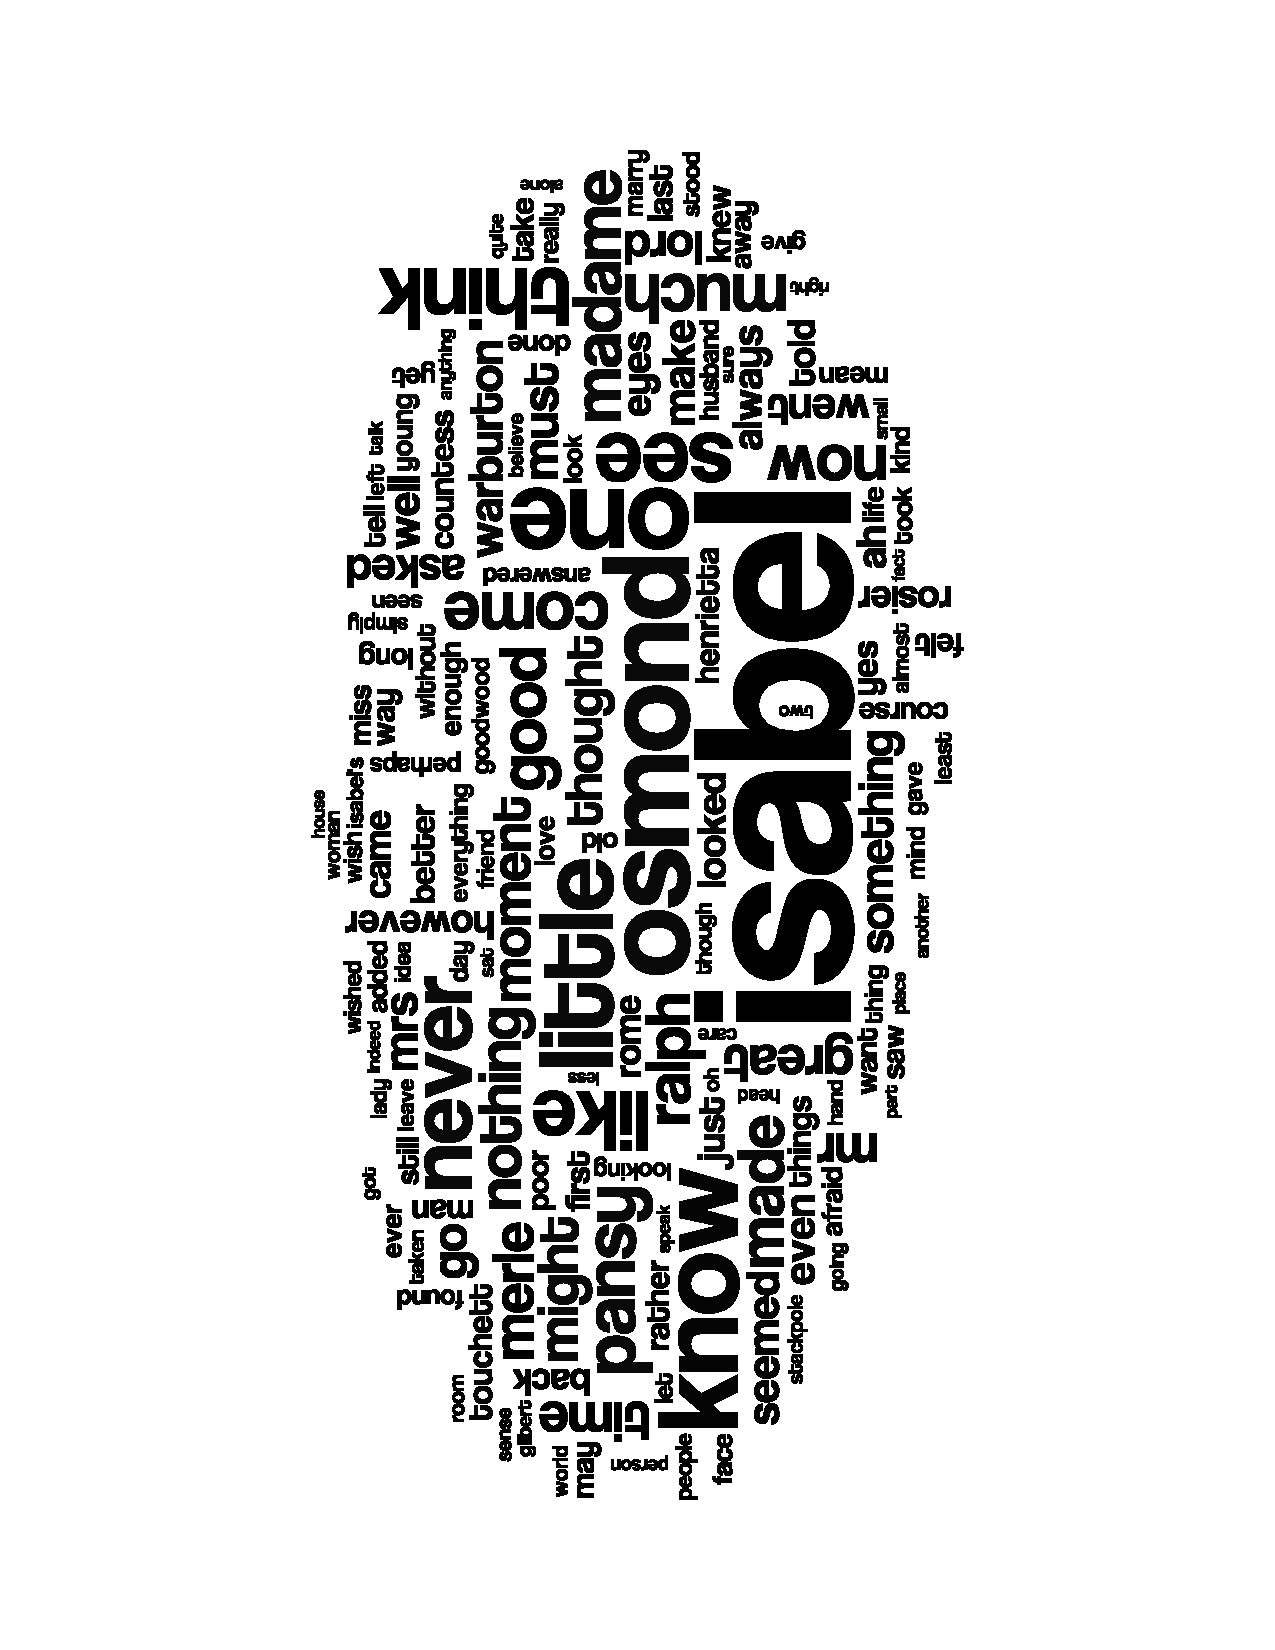
\includegraphics[angle=270,width=0.8\columnwidth]{resources/wordclouds/PortraitOfALady2_WordCloud.pdf}%
					\end{center}
					\caption{Word cloud for \emph{Portrait of a Lady Volume 2}}%
					\label{wcLadyTwo}%
				\end{figure}
				\begin{figure}[htb] 
					\begin{center}
					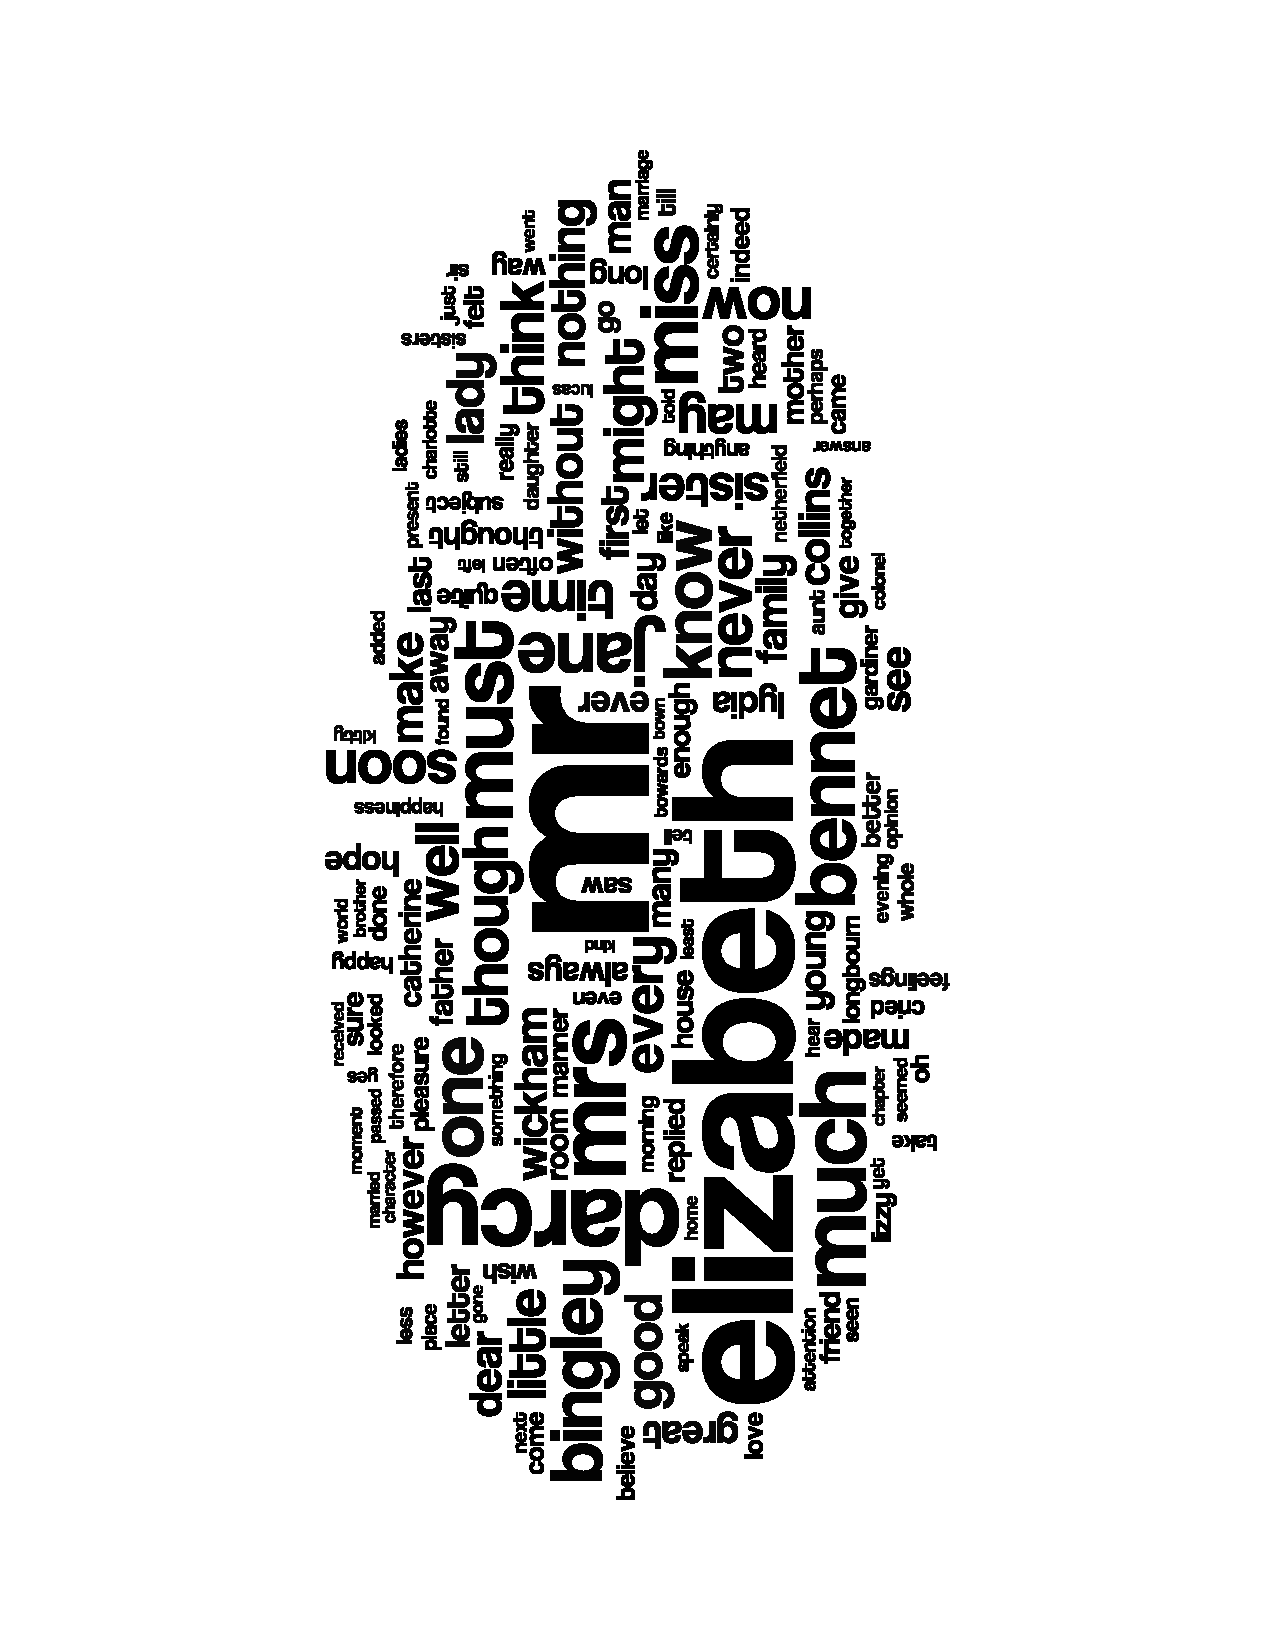
\includegraphics[angle=270,width=0.8\columnwidth]{resources/wordclouds/PrideAndPrejudice_WordCloud.pdf}%
					\end{center}
					\caption{Word cloud for \emph{Pride and Prejudice}}%
					\label{wcPride}%
				\end{figure}
				\begin{figure}[htb] 
					\begin{center}
					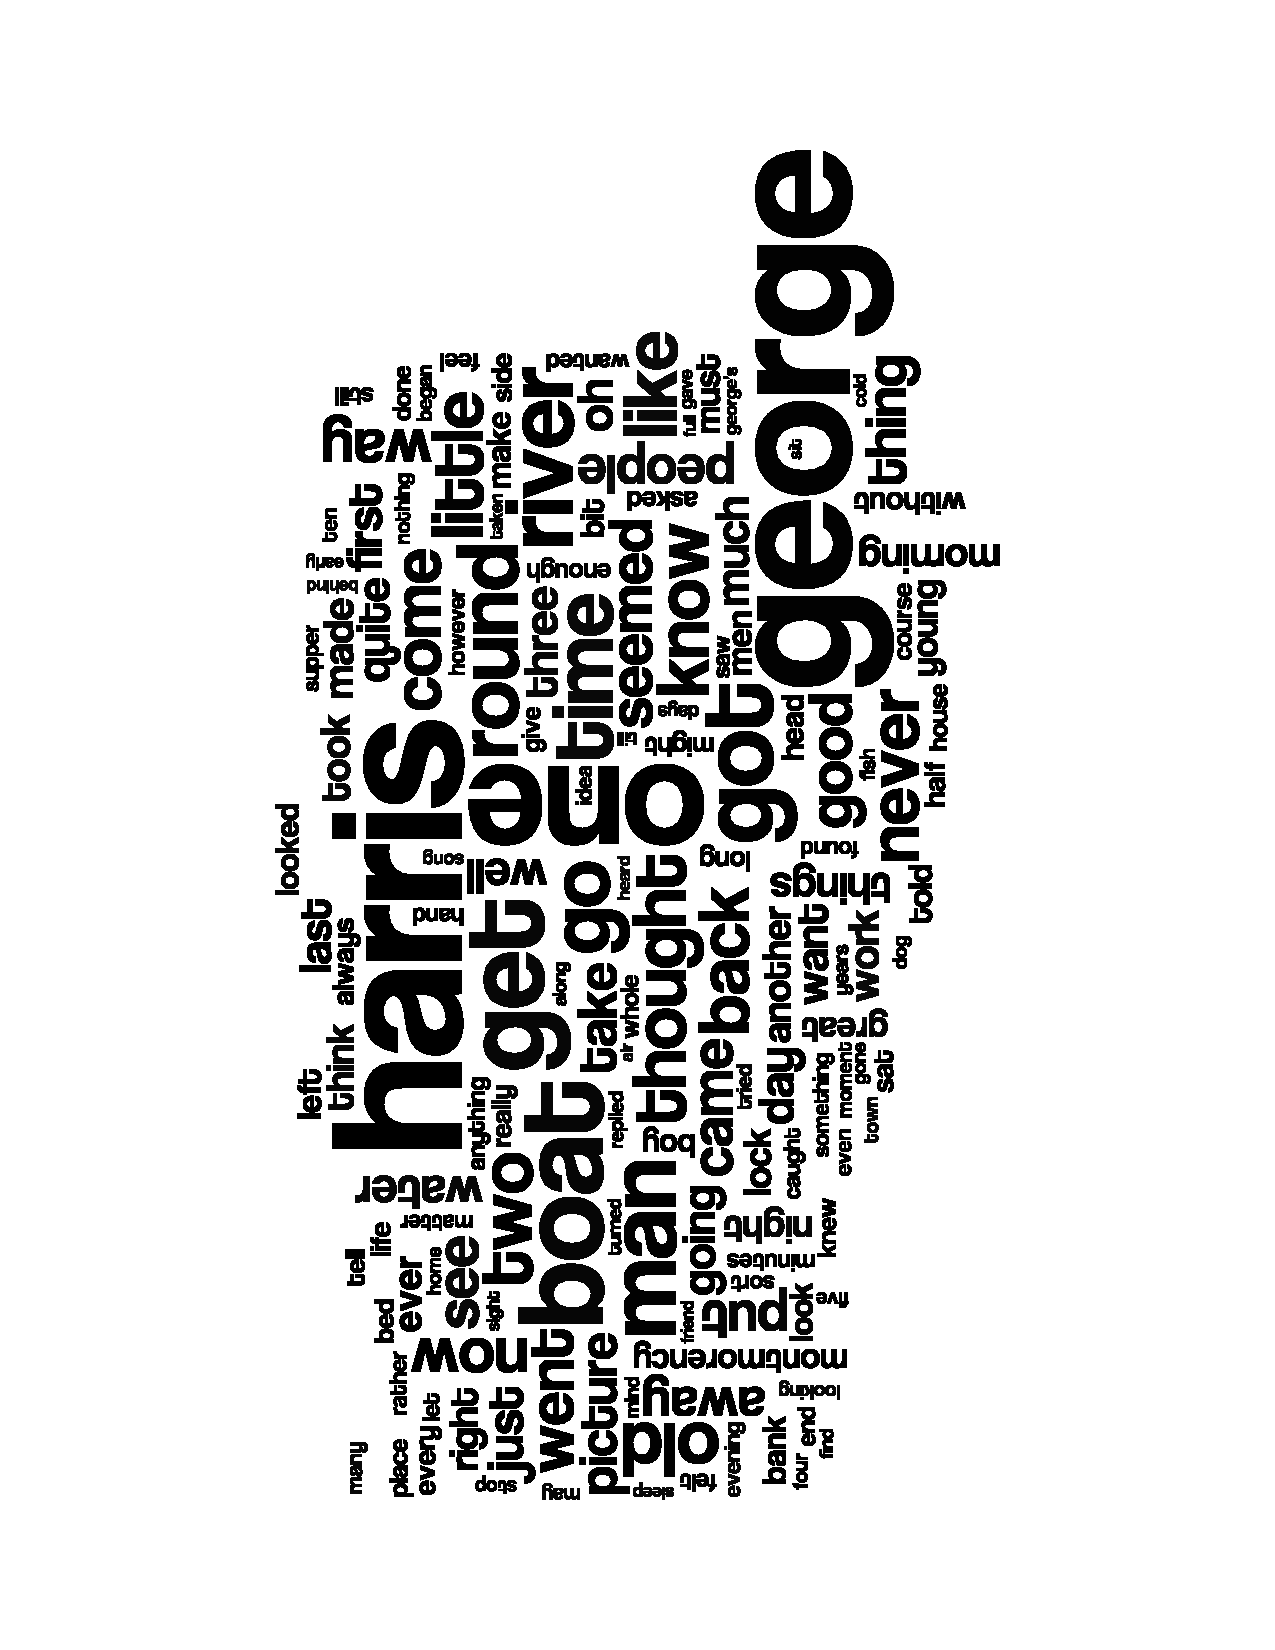
\includegraphics[angle=270,width=0.8\columnwidth]{resources/wordclouds/ThreeMenInABoat_WordCloud.pdf}%
					\end{center}
					\caption{Word cloud for \emph{Three Men in a Boat}}%
					\label{wcBoat}%
				\end{figure}
\end{enumerate}



\end{document}
